
\begin{figure}[h]
    \centering
    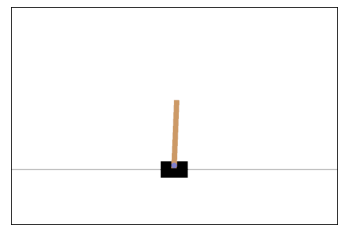
\includegraphics[width=0.7\textwidth]{Images/CartPole.png}
    \caption{Example of the rendered environment for the cartpole. We can notice the cart in black, the pole in brown and the moving rail represented by 
    black line.}
    \label{fig:Cart}
\end{figure}

\begin{figure}[h]
    \centering
    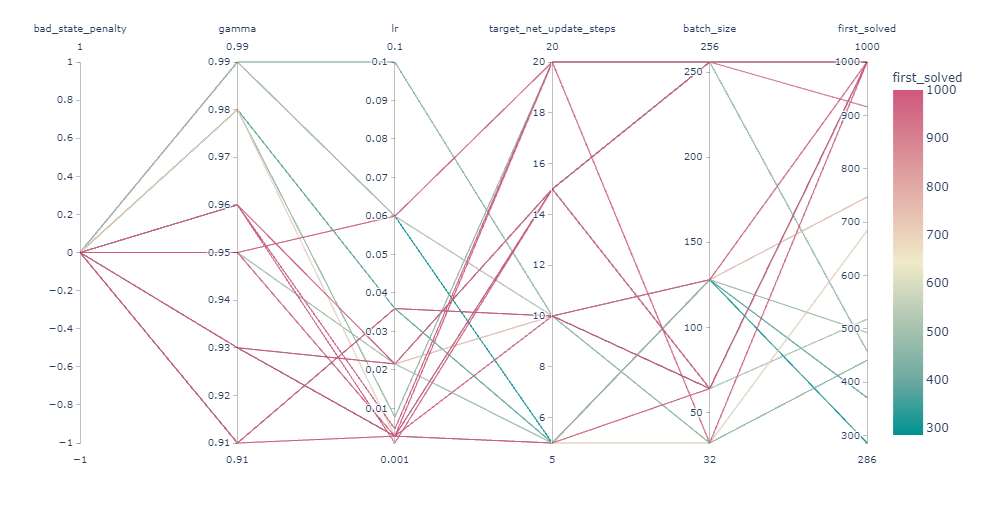
\includegraphics[width=\textwidth]{Images/CartPoleHyper2.png}
    \caption{Hyperparameters search, where the color of the line is proportional to the first\_solved field. 
        We stress that the best set of trials are the one with lowest first\_solved.}
    \label{fig:hyper}
\end{figure}

\begin{figure}[h]
    \centering
    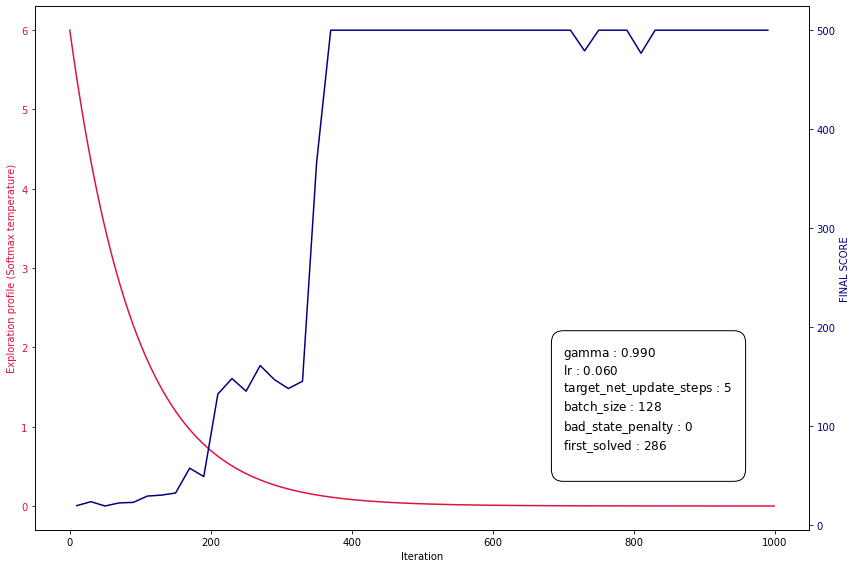
\includegraphics[width=0.7\textwidth]{Images/Best_set_Cartpole.png}
    \caption{In red the exploration profile and in blue the training score for the best performing hyperparameter set.
        The training score increases immediately after the temperature approaches $0$.}
    \label{fig:best_cart}
\end{figure}

\begin{figure}[h]
    \centering
    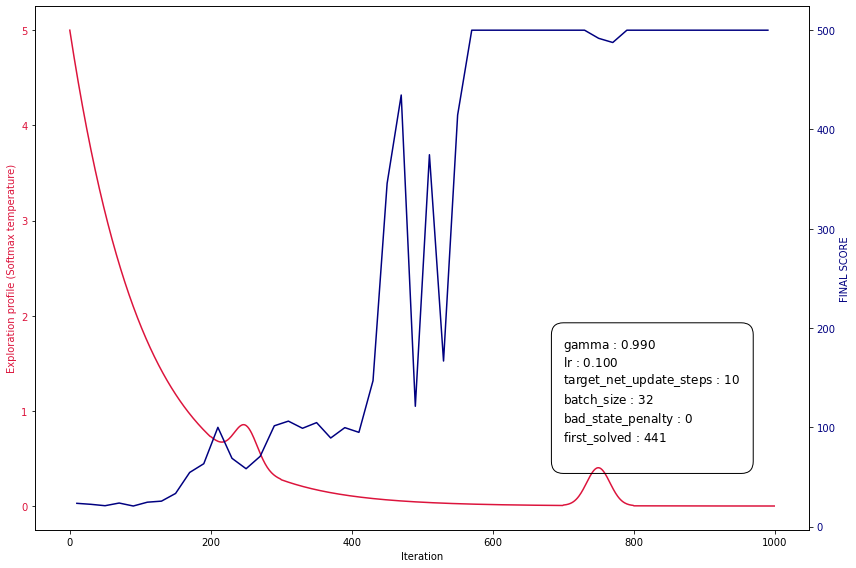
\includegraphics[width=0.7\textwidth]{Images/Good_Cartpole.png}
    \caption{In red the exploration profile and in blue the training score for a well performing hyperparameter set.
        We see that, even if we have an increase in the temperature towards the end, the agent still performs a very good score.}
    \label{fig:norm_cart}
\end{figure}

\begin{figure}[h]
    \centering
    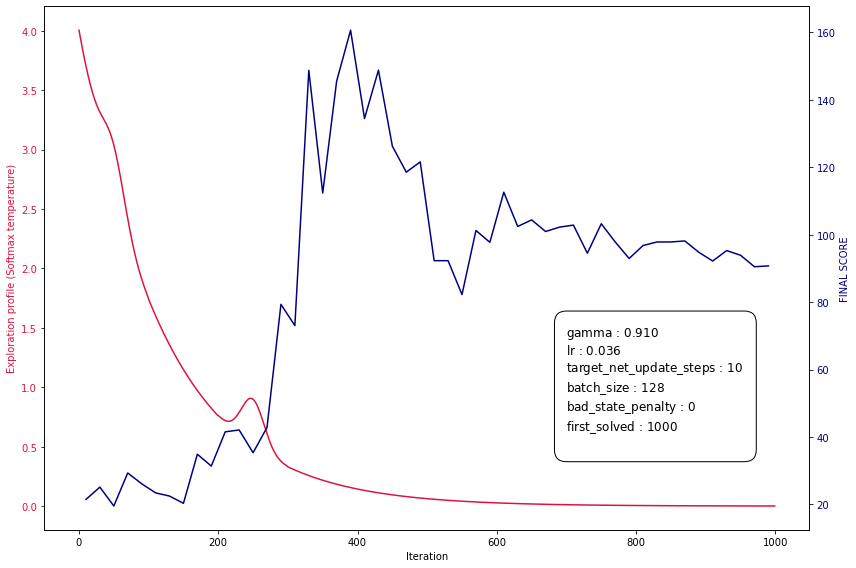
\includegraphics[width=0.7\textwidth]{Images/Bad_Cartpole.png}
    \caption{In red the exploration profile and in blue the training score for a hyperparameter set not able to solve the environment.
        The training score stabilizes around $100$, which is far under the maximum score.}
    \label{fig:bad_cart}
\end{figure}

\begin{figure}[h]
    \centering
    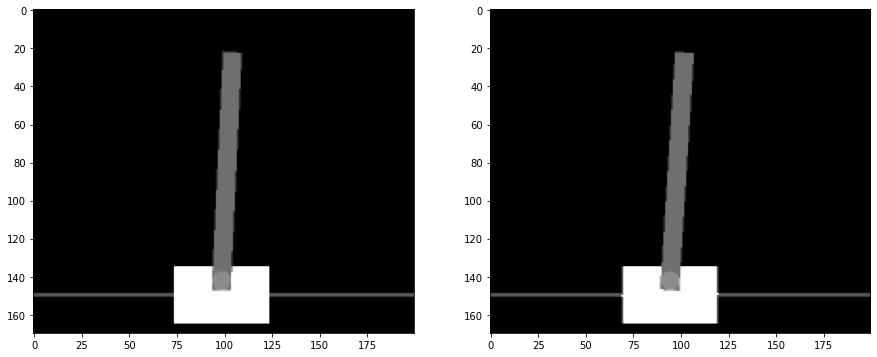
\includegraphics[width=0.7\textwidth]{Images/Sample_Cart_Image.png}
    \caption{Samples of the image given as an input to the network. We observe that they are cropped and putted in a grayscale.}
    \label{fig:image}
\end{figure}

\begin{figure}[h]
    \centering
    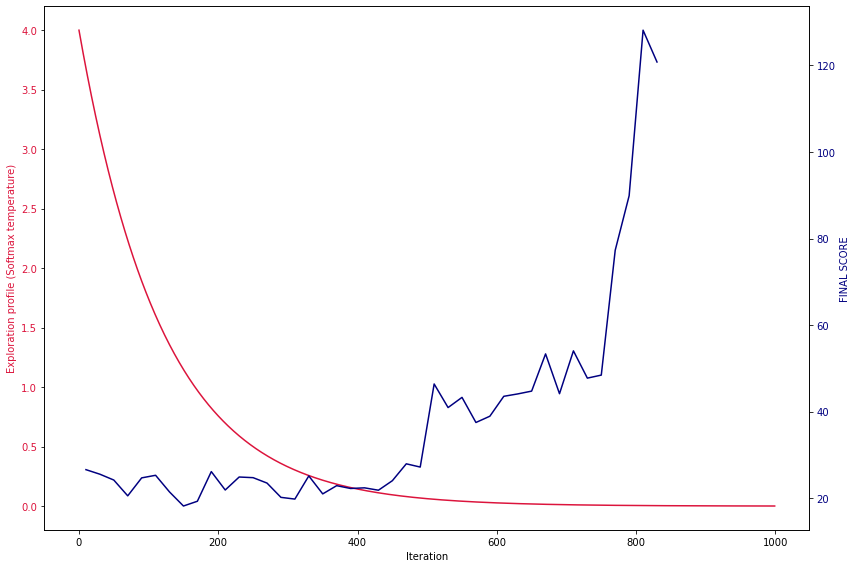
\includegraphics[width=0.7\textwidth]{Images/Pix_Prof_Before_trick.png}
    \caption{In red the exploration profile and in blue the training score before the application of the supervised network for the learning
        from pixels. The blue curve ends prematurely due to a memory leak. We can see that, even if the environment is not solved, the agent
        learns a strategy, since the average score increases significantly.}
    \label{fig:bef_trick}
\end{figure}

\begin{figure}[h]
    \centering
    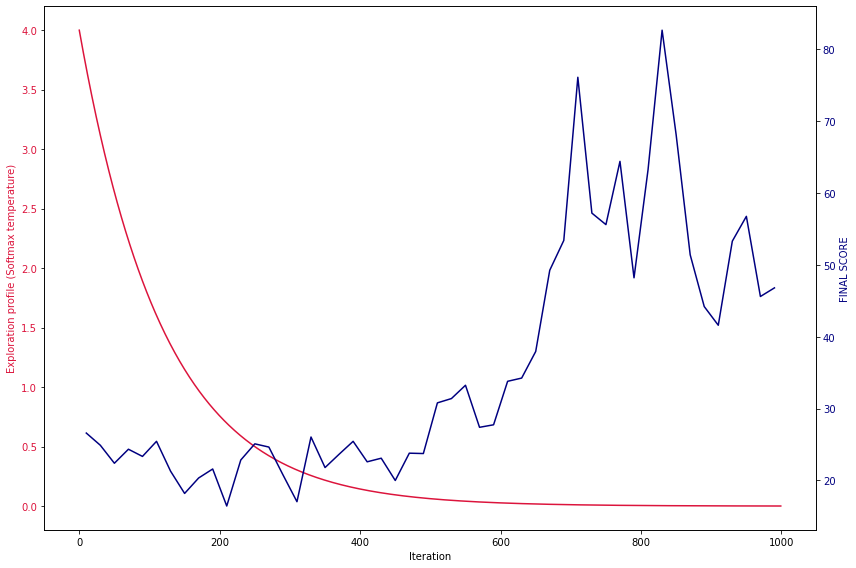
\includegraphics[width=0.7\textwidth]{Images/Pix_Prof_after_trick.png}
    \caption{In red the exploration profile and in blue the training score before the application of the supervised network for the learning
    from pixels. The score is lower than the one in Figure \ref{fig:bef_trick}. This is due to problems in the supervised learning task, such as
    the low number of training samples.}
    \label{fig:aft_trick}
\end{figure}

\begin{figure}[h]
    \centering
    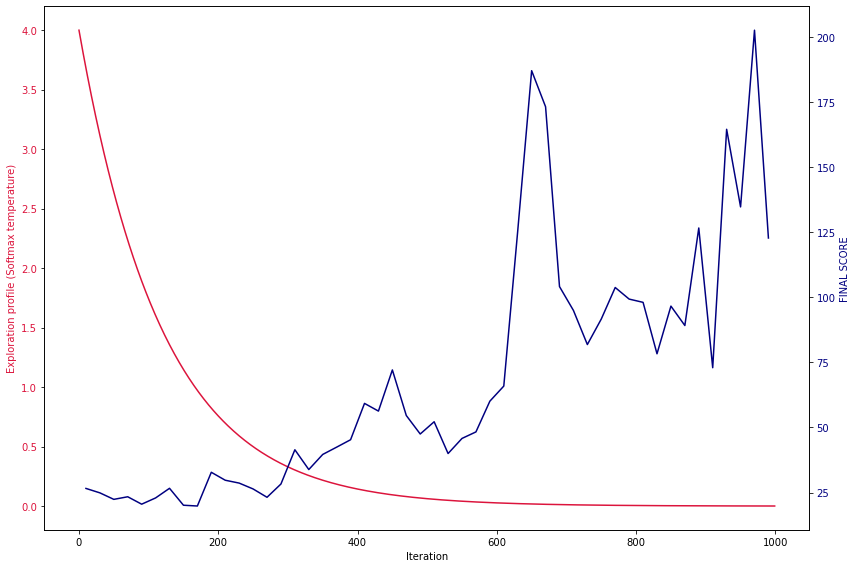
\includegraphics[width=0.7\textwidth]{Images/nofreeze.png}
    \caption{In red the exploration profile and in blue the training score, starting the learning from the supervised network 
    without freezing the weights. The score is higher than the one in Figure \ref{fig:bef_trick}, but it is really unstable and it so not a reliable
    improvement.}
    \label{fig:nofreeze}
\end{figure}

\begin{figure}[h]
    \centering
    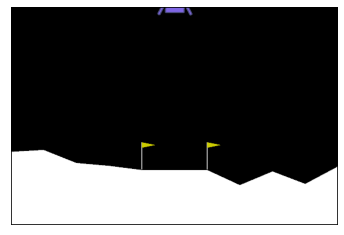
\includegraphics[width=0.7\textwidth]{Images/LunarLander.png}
    \caption{Example of the rendered environment for the lunar lander. We can notice the landing space delimited by the flags and the lander 
    in violet on the top center.}
    \label{fig:Lunar}
\end{figure}

\begin{figure}[h]
    \centering
    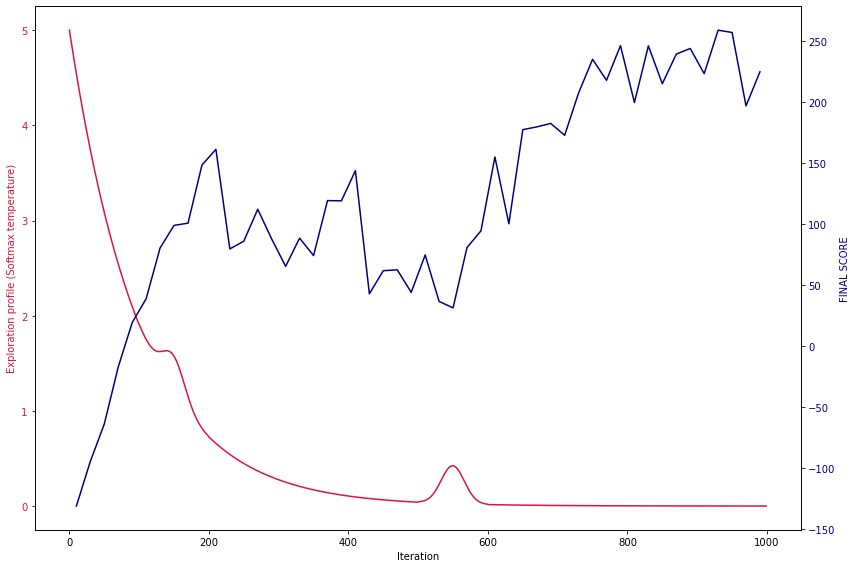
\includegraphics[width=0.7\textwidth]{Images/Lunar_Score.png}
    \caption{In red the exploration profile and in blue the training score for the LunarLander environment. 
    The environment is considered solved with a score of $200$, which is reached at around $800$ iterations. We can also observe that the score increases significantly at $600$ iterations after
    a plateau, in correspondence to the end of the gaussian addition.}
    \label{fig:score_lunar}
\end{figure}